\chapter{Apéndices} %%

\section{Observaciones / Notas} %

\begin{enumerate}
	\item La matriz \verb+ mat_posibles_url+ se define con un tamaño fijo antes de correr el algoritmo para que no se demore por tener un objeto que va cambiando de tamaño, por lo que al final de haberle aplicado la función se le deben de quitar los renglones que no tienen información.

  \item La función \textit{casos\_alumnos} convierte los \textit{NA} de la columna \textit{Alumnos} de \textit{m\_grande} en ceros pero al generar \textit{m\_grande\_total} y pasarla por la función \textit{limpia\_m\_grande} se eliminan los \textit{NA} y se cambian por ceros por lo tanto no es necesaria la función \textit{casos\_alumnos}, basta pasar la columna correspondiente a \textit{Alumnos} de \textit{m\_grande\_total}.
  
  \item Cuando se hacen comparaciones se toman los valores reales y se les restan los valores simulados $(Reales - \mathbb{E}[Simulados])$

  \item Con las gráficas \textit{heatmap} se revisa si el modelo es adecuado o si se debe modificar algo. Se espera que las gráficas sean de color claro ya que nos interesa que el número de grupos y alumnos simulados se parezca al real.
  
  \item Se tienen dos tipos de matrices las cuales llamaremos \textit{m\_objetivo} y \textit{m\_definición}; las matrices \textit{m\_objetivo} son las que tienen la información que se utiliza para la asignación; las matrices \textit{m\_definición} nos sirven para dos cosas:
  
	\begin{enumerate}
		\item Respaldo de la descripción de cada columna
		
		\item Para guardar los índices en los que se encuentran las columnas
	\end{enumerate}
  
%  \item Para obtener lo índices de las columnas de las matrices tipo \textit{m\_definición} se debe buscar el nombre en la columna 1 (de \textit{m\_definición}) y se debe arrojar un número de columna el cual se toma de la columna 2 (de \textit{m\_definición}), ese valor es el que se utiliza para sacar información de \textit{m\_grande}. 
  
  \item Las matrices tipo \textit{m\_definición} son:
  
  	\begin{enumerate}
  		\item mat\_def\_columnas\_MG
		
		\item mat\_def\_grupos\_reales
		
		\item mat\_def\_grupos\_simulados
	\end{enumerate}
  
  \item Las matrices tipo \textit{m\_objetivo} son:
  
  	\begin{enumerate}
  		\item m\_grande
		
		\item m\_grande\_total
		
		\item $\ldots$
	\end{enumerate}  
  
  
  \item La función \textit{checa\_ind\_materia} se encarga de obtener lo índices de las columnas de las matrices tipo \textit{m\_definición} para poder sacar información de \textit{m\_grande} o de \textit{m\_grande\_total}.
  
  \item Para las simulaciones se utiliza la información anterior a la del semestre que se quiere simular para no tener información real dentro  de los datos para la simulación.
  
  \item En caso de querer elegir la capacidad del salón se va a elegir la mayor de sus capacidades (comparando las capacidades que se han tenido a lo largo de varios semestres).
  
  \item Las matrices \textit{m\_grande} y de \textit{m\_grande\_total} tienen información real.
  
%  \item Al actualizar los renglones de \textit{m\_grande} sólo se se registran los horarios y salones en los que los profesores imparten su clase, no se toman en cuenta las clases impartidas por los ayudantes.
%  
%  Ej. \url{http://www.fciencias.unam.mx/docencia/horarios/20181/2055/1323}
%  
%  El profesor imparte su clase los lunes, miércoles y viernes de 13-14hrs en el salón O215, hay una ayudantía los martes y jueves de 13-14hrs en el salón O215 y otra ayudantía los martes de 11-13hrs en el salón 304 (Yelizcalli).
%  
%  Se considera que esta materia inicia a las 13hrs y se imparte en el salón O215.
%  
%\begin{figure}[H]
%\centering
%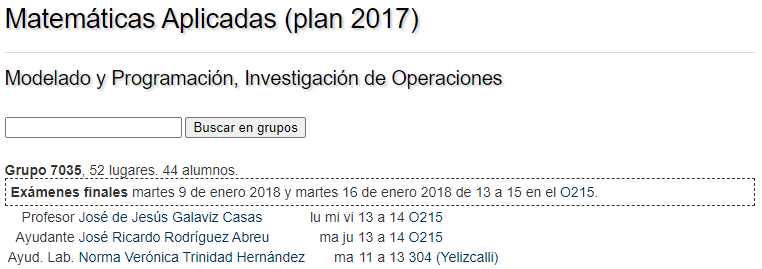
\includegraphics[scale = 0.65]{Ej_gpo_horarios_multiples} %width=\textwidth
%\caption{\textit{Ejemplo de grupo con horarios múltiples}}
%\end{figure}

  \item En los ciclos que recorren renglones y columnas de matrices, siempre es más rápido hacer (de afuera hacia adentro) primero las columnas y luego los renglones.
  
  Si se tiene una matriz con entradas $(i,j)$ entonces:
  
  \begin{lstlisting}[language=R, caption= \textit{Ejemplo de ciclo for}]
	for(j){
	 for(i){
      m[i,j]
    }
   }
  \end{lstlisting}

%\item[-] Las materias de inglés no se imparten todos los días de la semana, en algunos casos se imparten clases en línea; los días en que se imparten las clases presenciales se van a colocar en la columna \textit{Horario} para que sólo haya números en la columna \textit{horario\_num}.

  \item El vector \textit{vec\_nom\_materias\_total} tiene los nombres de las materias, sin repeticiones, que se utiliza para las simulaciones.
  
  \item El vector \textit{vec\_excepciones} tiene las posibles ecxepciones en las que las funciones que extraen información pueden caer, de esta manera se pueden generar nuevas funciones para corregir esos casos.
  
  \item La siguiente imagen es el resultado de la función \textit{imprime\_info\_idiomas} la cual muestra la información de los idiomas. Dicha función arroja un vector con los semestres que requieren modificación.

\begin{figure}[H]
\centering
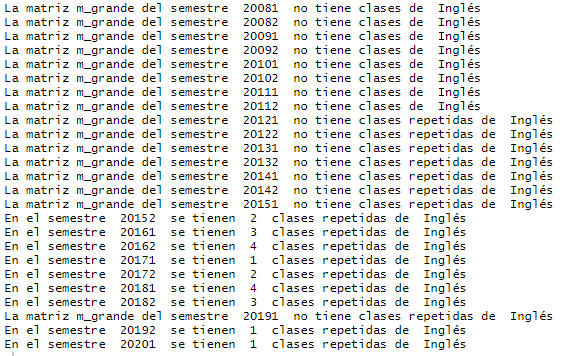
\includegraphics[scale = 0.65]{clases_de_ingles} %width=\textwidth
\caption{\textit{Resumen de clases de ingles antes de modificación}}
\end{figure}  
  
Con esta información se decidió observar caso por caso los renglones que requieren modificación para la matriz \textit{m\_grande}


  \item Debido a la situación en la que estamos viviendo actualmente, ahora más que nunca es necesario tener un programa para la asignación de horarios que permita la realización de las asignaciones sin tener la necesidad de hacer reuniones en persona, ya que al proseguir con las medidas de distanciamiento social, las reuniones antiguamente hechas en persona se tendrían que hacer por medio de alguna plataforma digital las cuales no necesariamente son las más óptimas ya que dependen de la señal de todos los participantes para que haya una comunicación de manera fluída. Debido a ésto, el programa es una buena solución.

  \item Al hacer las simulaciones del número de alumnos el redondeo es hacia arriba, usando la función \textit{ceiling}.
  
  \item El vector \textit{vec\_nom\_materias\_total}, que contiene el nombre de las materias se definió en la lista \textit{param} para poder tomarlo en las diferentes funciones.
  
  \item Para resolver un problema, pensar en los pasos en los que se puede dividir dicho problema, usualmente se requieren entre 3 y 8 pasos o casos para obtener un producto final. Para cada paso hacer una función. 
  
  Se tienen dos posibles estructuras:
  
  \begin{itemize}
  \item[a)] La función del paso $n$ manda a llamar a la del paso $n-1$.
  
  Ej.

  $\textit{simula\_grupos} \left\{ \textit{simula\_gpos\_1\_sem}\right. \left\{ \textit{simula\_gpos\_1\_materia}\right. \left\{ \textit{simula\_tam\_gpo}\right.$\\
  
  \item[b)] Se tiene una función principal que manda a llamar a las funciones de cada paso:
  
  Ej.

%  \begin{lstlisting}[language=R, caption= Ejemplo 2 de estructura de funciones]
  \begin{lstlisting}[language=R, caption= \textit{Ejemplo de estructura de funciones}]
  gen_asignacion_completa <- function(sem_ini,sem_fin){   
    # Se carga y se limpia la lista de urls (para no tener paginas sin informacion,...)
    list_url <- Actualiza_list_url(list_url)
    
    # Se obtiene "m_grande" y se genera un archivo para cada semestre
    for(k in 1:length(semestres)){
      sem_info <- semestres[k]
      directorio_info[k] <- gen_m_grande(sem_info,list_url)
    }
    
    # Se genera el esqueleto del semestre que se quiere obtener
    mat_esqueleto <- gen_esqueleto(directorio_info,param)
        
    # Se genera la matriz de solicitudes de todos los profesores
    mat_solicitudes <- gen_solicitudes(param)
    
    # Se genera la matriz de asignaciones de todos los profesores
    mat_asignaciones <- gen_asignacion(mat_esqueleto,mat_solicitudes,param)
    
    return(mat_asignaciones)
  }
}
  \end{lstlisting}
  \end{itemize}
  
  \item Pudiera ser que haya un apéndice con ``Observaciones'' utlizando las notas escritas.
  
  \item Todo lo que se escriba debe tener un propósito, sino quitarlo.
  
  \item La información que se puede encontrar actualmente (debido a la pandemia) en las páginas web de los horarios de la FC no es la misma que la mostrada a lo largo del trabajo ya que ahora no se tiene información del salón, o del número de alumnos inscritos por materia, ni los lugares disponibles por grupo.
  
\begin{figure}[H]
\centering
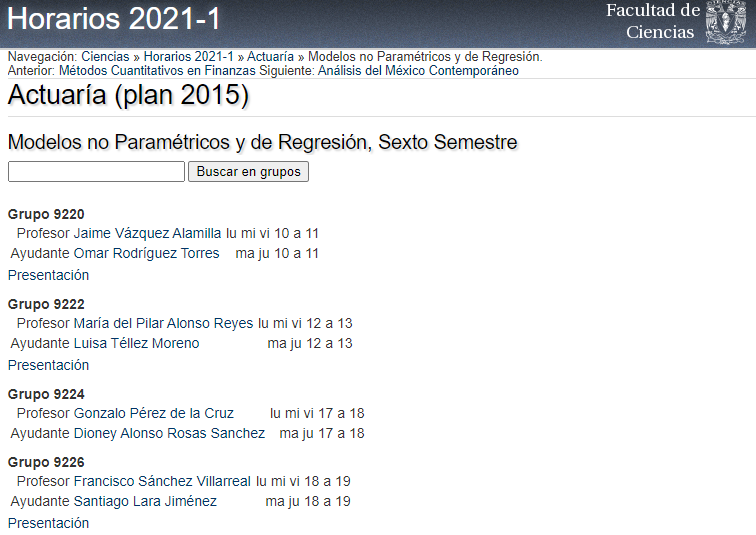
\includegraphics[scale = 0.45]{Ej_horarios_20211} %width=\textwidth
\caption{\textit{Ejemplo de horarios de semestre 2021-1}}
%\url{http://www.fciencias.unam.mx/docencia/horarios/20211/2017/1639}
\end{figure}
  
  \item Notas de T26
\begin{figure}[H]
\centering
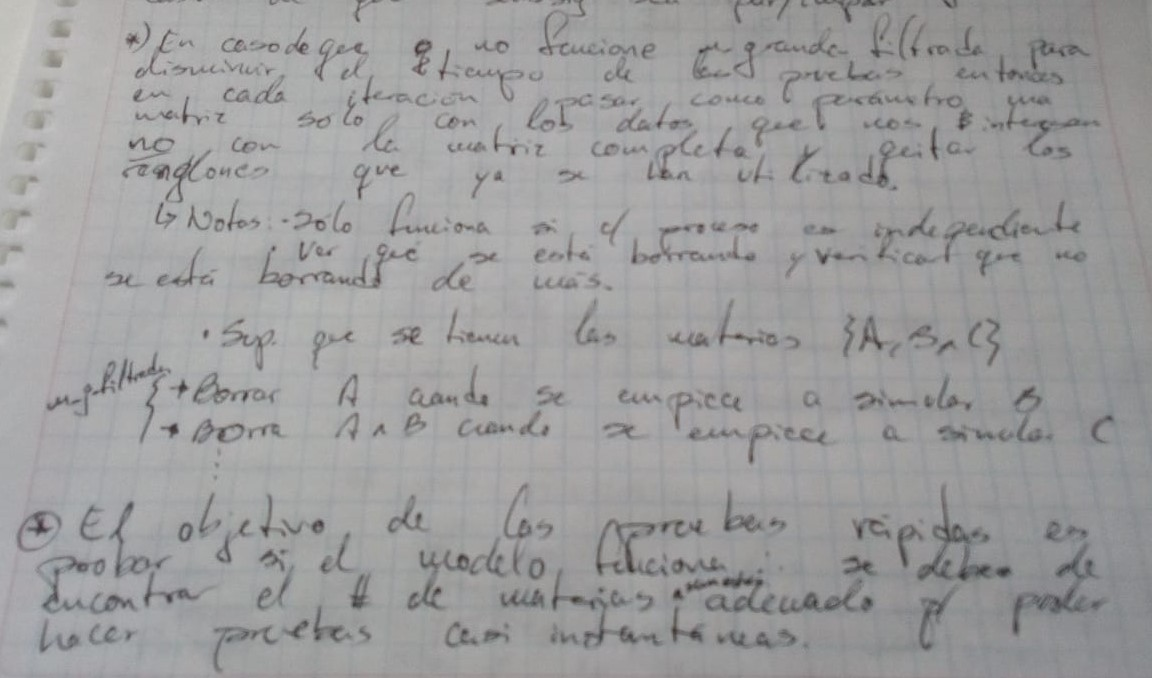
\includegraphics[scale = 0.4]{Notas_T26} %width=\textwidth
\caption{\textit{Notas de T26}}
\end{figure}
  
  \item En caso de tener subsecciones: entre 3 y 4
  
  \item La estructura de cada párrafo debe ser de tipo \textit{reloj de arena}. Ir de lo general a lo particular y volver a lo general con una conclusión.
  
  \item Sea $D = \dfrac{r - s}{s}$, donde \textit{r} son datos reales, \textit{s} datos simulados y \textit{D} la diferencia relativa, se busca que $D \in \left[ -\dfrac{1}{2},\dfrac{1}{2}\right]$. 
  
  \item Ejemplo del uso del comando \textit{Roxygen} para comentar las funciones en \textit{R}.
\begin{figure}[H]
\centering
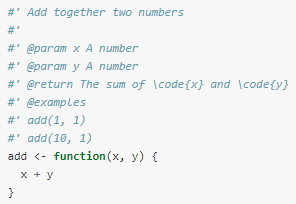
\includegraphics[scale = 1]{Ej_Roxygen} %width=\textwidth
\caption{\textit{Ejemplo de Roxygen}}
\end{figure}
  
  \item Escribir en el archivo de LaTeX pequeños comentarios de la idea que se quiere transmitir en cada párrafo (de 2 a 3 palabras claves). Ésto sirve para referencias futuras y para ordenar los párrafos con mayor facilidad.
  
  \item Escribir párrafos de 2 a 3 enunciados completos, no dejar enunciados solos a menos que contengan información muy importante.
  
  \item En caso de tener más de 10 referencias bibliográficas utilizar \textit{Mendeley} para genera un archivo \textit{.bib} y  ponerlo en la tesis para tener la bibliografía.
  
  \item Cuidar el tamaño de letra en las gráficas que se pongan
  
  \item No poner abreviaturas en los títulos.
  
  \item Ser muy directa al escribir, pero explicar mucho más (platicar más). No hacer enunciados tan largos. Escribir una idea por enunciado. No sólo escribir en párrafos, utilizar listas, tablas, ...
  
  \item La imagen \ref{img_en_ing_2} tiene título en inglés, se tienen 2 opciones: dejarlo así o buscar cómo cambiarlo.
  
  \item Recordar la diferencia entre:
  \begin{itemize}
  	\item[-] Número de alumnos inscritos
  	
  	\item[-] Número de alumnos reales
  	
  	\item[-] Número de alumnos que toman clase por cada horario (no se toman en cuenta los alumnos que empalman clases)
  \end{itemize}
  
  \item Para la elección de $q_{1}$ y $q_{2}$ se debe darle prioridad a la varianza no al mín y al máx porque se pueden tener casos en los que el mín y el máx estén muy cercanos a cero (gráfica superior) pero su varianza es grande. Queremos que la varianza se encuentre alrededor del cero (gráfica inferior).

\begin{figure}[H]
\centering
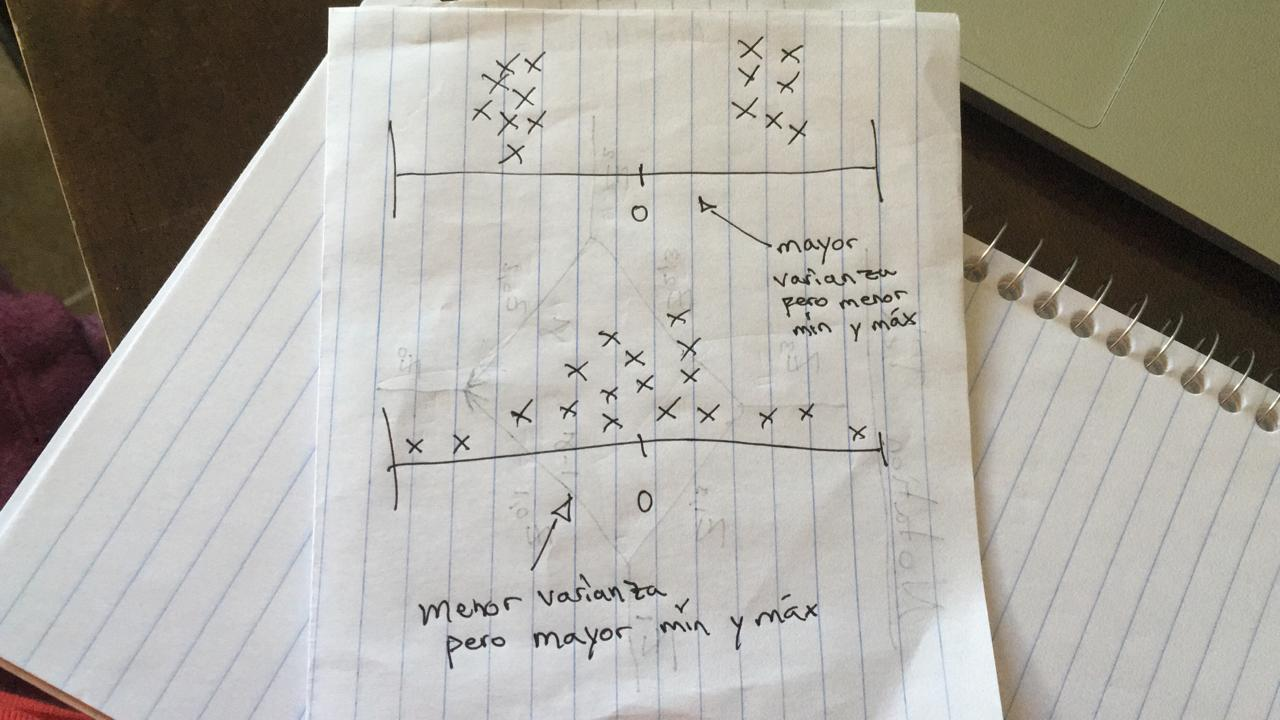
\includegraphics[scale = 0.3]{Ej_varianza} %width=\textwidth
\caption{\textit{Ejemplo de varianza}}
\end{figure}
  
  \item Preferir sacrificar el B/N en las imágenes impresas para tener una mejor versión digital a color.
  
  \item Guardar figuras hechas en R con el comando: \textit{dev.print(pdf, ``Figures/Fig\_Examples\_of\_GB\_distributions.pdf'',width=8, height=5)}
  
  \item Arrigo dijo que posiblemente alguien se va a quejar de no tomar en cuenta la preferencia de los profesores al realizar las solicitudes.
  
  \item Un histograma nos muestra la representación de la distribución empírica de un conjunto de datos. Cada barra en el histograma representa la frecuencia de un intervalo sobre el rango de las observaciones que se tienen.
  
  \item Cláusula 99 CCTPA: Ayuda para la impresión de la tesis.
  
  \url{https://www.personal.unam.mx/Docs/Contratos/AAPAUNAM20132015.pdf}

\begin{figure}[H]
\centering
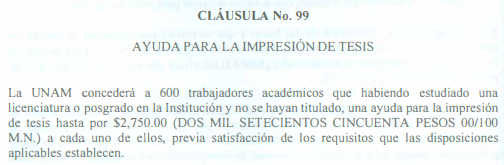
\includegraphics[scale = 0.8]{clausula99_CCTPA} %width=\textwidth
\caption{\textit{Cláusula 99 CCTPA: Ayuda para la impresión de la tesis}}
\end{figure}
  
  \item Equivalencias de nombres para estadística:
  \begin{enumerate}
  \item Estadística I - Inferencia Estadística
  
  \item Estadística II - Modelos no Paramétricos y de Regresión
  
  \item Estadística III - Modelos de Supervivencia y de Series de Tiempo
  \end{enumerate}
  
  \item La frecuencia relativa en los histogramas no refleja directamente el porcentaje. Se debe multiplicar el valor del eje $Y$ por el ancho del intervalo por $100$ para obtener cifras en porcentaje. El área total de las barras sumará 1 (\ref{MargaritaJaimeRuthLizbeth}).
  
  \item No confundir las carpetas de \textit{Figuras} del GitHub con la del pdf.
  
  \item Ya no son necesarias las pruebas de bondad de ajuste porque los tamaños de grupo se van a simular con respecto a los profesores. Ver $T_{32} xx)$
  
  \item 
  
  \item 
  
  \item 
  
  \item 
  
  \item 
\end{enumerate}


\section{Resultados útiles} %

\begin{defn} \label{EMVlambda}
\textbf{Estimador máximo verosímil de $\lambda$}

Sean $X_{1}, X_{2}, \ldots, X_{n}$ una muestra aleatoria de una población con función de densidad de probabilidad $Poisson(\lambda)$. Su función de densidad es:

\begin{equation}
f(x) = \mathrm{e}^{-\lambda} \dfrac{\lambda^{x}}{x!}
\end{equation}

\begin{eqnarray*}
\mathcal{L}(X_{1}, X_{2},\ldots, X_{n}; \lambda) &=& \displaystyle \prod_{i = 1}^{n} \left( \mathrm{e}^{-\lambda} \dfrac{\lambda^{x_{i}}}{x_{i}!} \right)\\
												 &=& \mathrm{e}^{-n \lambda} \dfrac{\lambda^{\displaystyle \sum_{i = 1}^{n} x_{i}}}{\displaystyle  \prod_{i = 1}^{n} x_{i}!}\\
\text{Sacamos ln}\\
ln \mathcal{L}(X_{1}, X_{2}, \ldots, X_{n};\lambda) &=& -n\lambda + \displaystyle \sum_{i = 1}^{n} x_{i} ln \lambda - ln \displaystyle  \prod_{i = 1}^{n} x_{i}! \\
\text{Derivamos con respecto a } \lambda\\
\dfrac{\partial}{\partial \lambda} ln \mathcal{L}(\underline{X};\lambda) &=& -n + \dfrac{\displaystyle \sum_{i = 1}^{n} x_{i}}{\lambda} \\
\text{Igualamos a cero}\\
-n + \dfrac{\displaystyle \sum_{i = 1}^{n} x_{i}}{\lambda} &=& 0 \\
\Rightarrow\\
\text{Despejamos } \lambda\\
\hat{\lambda} &=& \dfrac{\displaystyle \sum_{i = 1}^{n} x_{i}}{n} = \overline{x}\\
\text{Derivamos otra vez}\\
\dfrac{\partial^{2}}{\partial \lambda} ln \mathcal{L}(\underline{X};\lambda)  &=& - \dfrac{\displaystyle \sum_{i = 1}^{n} x_{i}}{\lambda^{2}} < 0\\
\therefore \hat{\lambda} &=& \overline{x} \,\,\,\,\,\, \text{es el estimador máximo verosímil}
\end{eqnarray*}
\end{defn}







\section{Abreviaturas} %
%\begin{itemize}
%\item CdC:= Ciencias de la Computación
%
%\item FC:= Facultad de Ciencias de la UNAM
%
%\item MatAp:= Matemáticas Aplicadas
%
%\item UNAM:= Universidad Nacional Autónoma de México
%
%\item  URL:= Uniform Resource Locator
%\end{itemize}


\begin{table}[H]
\centering
\begin{tabular}{|c|c|}
\hline 
 ABREVIATURA & SIGNIFICADO \\ 
\hline 
 CdC & Ciencias de la Computación \\ 
\hline 
 ESIME & Escuela Superior de Ingeniería Mecánica y Eléctrica\\ 
\hline 
 FC & Facultad de Ciencias de la UNAM \\ 
\hline 
 FES & Facultad de Estudios Superiores \\
\hline 
 ITAM & Instituto Tecnológico Autónomo de México \\ 
\hline 
 MatAp & Matemáticas Aplicadas \\ 
\hline 
 UNAM & Universidad Nacional Autónoma de México \\ 
\hline 
 URL & Uniform Resource Locator \\ 
\hline 
 a & b \\ 
\hline 
\end{tabular} 
\caption{\textit{Abreviaturas}}
\end{table}

